\section{Gaussian Processes}
\framecard{\insertsection}

\subsection{Recap}
\begin{frame}{\insertsubsection}
    \framesubtitle{Linear Regression} 

    \textcolor{UniGold}{\textbf{What was done until here?}}
    \begin{itemize}
        \item We assumed that our targets $t$ were \textcolor{UniOrange}{\textbf{i.i.d.}} and given by $t = y(\mathbf{x}) + \varepsilon$, where $\varepsilon \sim \mathcal{N}(0,\beta)$.
        \item Our model is given by $\mathbf{y}(\mathbf{x}) = \Phi^T \mathbf{w}$, where $\Phi$ is the \textcolor{UniOrange}{\textbf{design matrix}}, and this caracterize our model as \textcolor{UniOrange}{\textbf{linear in parameters}}.
        \item The \textcolor{UniOrange}{\textbf{design matrix}} was defined as $ \phi_{i,j} = \phi_i(\mathbf{x}_j)$.
        \item The \textcolor{UniOrange}{\textbf{parameters}} were given by $\mathbf{w} = \left( \Phi^T \Phi \right)^{-1}\Phi^T \mathbf{t}$.
        \item These \textcolor{UniOrange}{\textbf{parameters}} calculated at the minimum of the cost function are called \textcolor{UniOrange}{\textbf{maximum likelihood}}.
    \end{itemize}
    \begin{columns}
        \begin{column}{0.5\linewidth}  
        \begin{center}
        \centering
        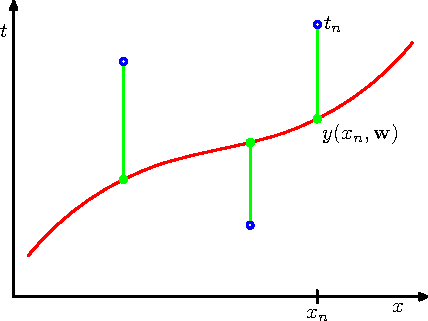
\includegraphics[width=0.9\linewidth]{Figure1c3.pdf}
         \end{center}
    \end{column}
    \begin{column}{0.5\linewidth}  %%<--- here
        \begin{center}
        \centering
        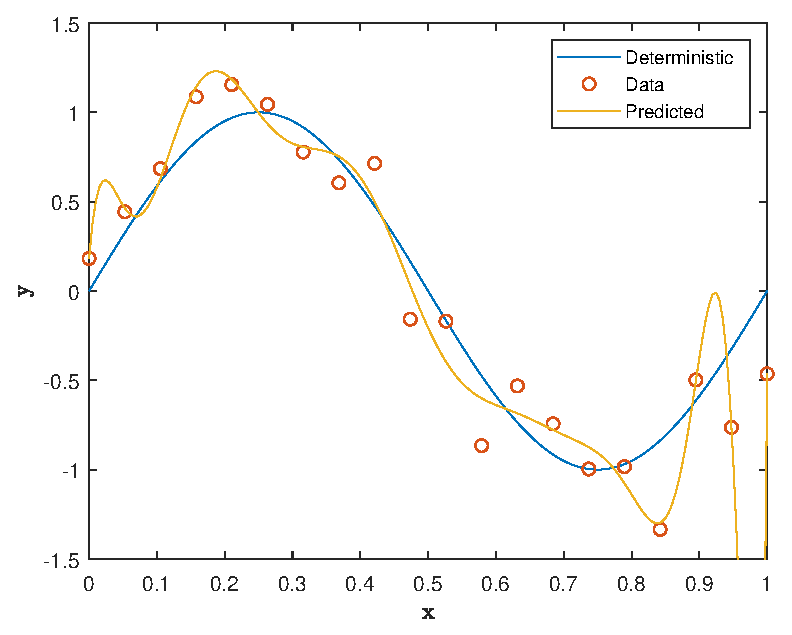
\includegraphics[width=0.9\linewidth]{lnReg.eps}
         \end{center}
    \end{column}
    \end{columns}

\end{frame}

\begin{frame}{\insertsubsection}
    \framesubtitle{Bayesian Linear Regression} 

    \textcolor{UniGold}{\textbf{What was done until here?}}
    \begin{itemize}
        \item We put an \textcolor{UniOrange}{\textbf{uncertainty}} over the targets $t$ and the parameters $\mathbf{w}$.
        \item We assumed that targets being \textcolor{UniOrange}{\textbf{distributed}} as $p( t| \mathbf{x}, \mathbf{w}, \beta) = \mathcal{N} ( t | y(\mathbf{x}, \mathbf{w}), \beta^{-1})$.
        \item This allowed to make an \textcolor{UniOrange}{\textbf{inference}} to obtain a \textcolor{UniOrange}{\textbf{prediction}} of the parameters.
        \item By \textcolor{UniOrange}{\textbf{Bayes' Rule}} we obtained that $p\left( \mathbf{w} | \mathbf{x}, \mathbf{t}, \alpha, \beta \right) \propto p\left(  \mathbf{t} |\mathbf{w} ,\mathbf{x}, \beta \right) p\left( \mathbf{w} | \alpha \right)$
    \end{itemize}

    \begin{figure}
		\label{fig:baReg}
        \hspace*{-1.4cm}\includegraphics[totalheight=0.3\textheight]{"baReg".eps}
	\end{figure}
\end{frame}

%%%%%%%%%%%%%%%%%%%%%%%%%%%%%%%%%%%%%%%%%%%%%%%%%%%%%%%%%%%%%%%%%%%%%%%%%%%%%%%%%%%%%%%%%%%%%
\subsection{Kernels}
\begin{frame}{\insertsubsection}
    
\end{frame}